\chapter{Embedded implementation}
\label{ch:Embedded}
In \autoref{ch:Framework}, an overview of the \gls{glo:frmwrk} developed in \texttt{\gls{glo:python}} was given, relying on the \gls{glo:mongodb} database. This chapter will focus on the implementation of the embedded system. The first big difference is that the embedded system is written in \texttt{C}, which is not an object-oriented language. The second big difference is that the embedded system does not use a database, but it relies only on the variables stored in the RAM. Because of the memory constraints, the training phase relies upon the communication with a \gls{pc} for storing the heavy data. Once the model has been trained, the model is stored in the embedded program and the novelty detection is performed in real time. The general structure is shown in \autoref{fig:Embedded}.

\begin{figure}
    \centering
    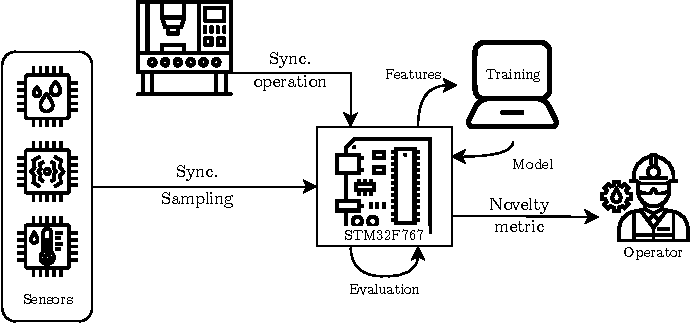
\includegraphics[scale=1]{images/Embedded/EmbeddedStructure.pdf}
    \caption{Embedded system overview}
    \label{fig:Embedded}
\end{figure}


\section{Hardware}
The hardware used for the implementation is the STM32F767ZI board. The characteristics of the board are resumed in \autoref{tab:stm32f767zi}.


\begin{longtable}{p{0.35\linewidth}p{0.55\linewidth}}
    \caption{Hardware characteristics of STM32F767ZI board}    \label{tab:stm32f767zi}\\
    \toprule
    \textbf{Feature} & \textbf{Description} \endfirsthead 
    \hline
    Microcontroller & STM32F767ZI \\
    Architecture & ARM Cortex-M7 \\
    Clock Speed & Up to 216 MHz \\
    Flash Memory & 2 MB \\
    SRAM & 512 KB \\
    EEPROM & No \\
    \gls{gpio} & Up to 176 \\
    Timers & 3 x 12-bit, 12 x 16-bit, 2 x 32-bit \\
    \gls{adc} & 3 x 12-bit \\
    DAC & 3 x 12-bit \\
    Communication Interfaces & USART, UART, SPI, I2C, CAN, Ethernet, USB \\
    Operating Voltage & 1.7V - 3.6V \\
    Operating Temperature & \SI{-40}{\celsius} to \SI{+150}{\celsius} \\
    \bottomrule    
\end{longtable}

Similarly to what has been done for the \texttt{\gls{glo:python}} implementation, the parameters of the algorithm are configurable. To avoid the reading of files during the operation, the configuration is held in global variables defined in a header file. The configurable parameters are the usual: depth of the wavelet three, number of \gls{glo:feature}s, sampling frequency, time-series length etc.

\section{Software}
The code consists of a main loop, that is continuously running. It is responsible for executing the state machine behaviour, that manages the different phases of operation. The phases of operation are the same as described for the \texttt{\gls{glo:python}} implementation, except for the training phase, in which the microcontroller performs the sensor \gls{glo:polling} and the \gls{glo:feature} extraction and then sends the data to the \gls{pc} using serial communication. The \gls{pc} is responsible for the training phase. This part is developed again in \texttt{\gls{glo:python}}, but the final model is then formatted as a \texttt{model.h} file that can be directly included in the embedded code. The model is then stored in the flash memory of the microcontroller, together with the rest of the program.

The hardware configuration has been done using the \gls{ide} ({STM32cubeIDE} tool), which is a graphical interface that allows the configuration of the microcontroller and generates the initialization code. 

\subsection{Sensor \gls{glo:polling}}
The microcontroller comes with a Hardware Abstraction Layer (\gls{hal}) which acts as an intermediary layer between the hardware and software. It simplifies interaction with the microcontroller's peripherals, such as \gls{gpio}, UART, and timers, by providing \gls{glo:std} functions and APIs. The \gls{hal} library enhances code reusability across different STM32 microcontroller families, streamlining the development process and enhancing the scalability of embedded systems projects.

To sample the data at a precise sampling frequency, two options are available:
\begin{itemize}
    \item Use the Direct Memory Acces (\gls{dma}) capability of the microcontroller. This approach allows sampling the \gls{gpio} and storing the result in the memory accessible by the CPU, without using CPU time. The \gls{dma} is then configured to trigger an interrupt at the end of the transfer, and the interrupt is used to signal the end of the sampling and to start the \gls{glo:feature} extraction. It is suitable for high sampling frequencies and in fact, even downscaling the clock frequency linked to the \gls{dma} there is a lower bound of obtainable sampling frequencies.
    \item Use the Timer peripheral of the microcontroller. The timer is configured to trigger an interrupt at a precise frequency, and the interrupt causes the CPU to poll the sensor data. This approach is suitable for sampling frequencies that are not too high, and it is the one used in this work (for frequency in the order of \SI{ }{\kilo\hertz}).
    If too many interrupts are generated, the CPU may not be able to execute them instantly, so the actual sampling may shift from the desired frequency, however, in this implementation the only interrupt used is the one for the sampling, so the CPU is not overloaded and the sampling frequency is precise.
\end{itemize}


\subsection{Feature extraction}
The \gls{glo:feature}s available to be extracted are the same as the ones described in \autoref{ch:FeatureExtraction}. The time-domain \gls{glo:feature}s are coded directly in a function that is responsible for extracting them. The frequency-domain \gls{glo:feature}s are computed by another function that relies on the \texttt{C} library \texttt{wavelib} for the wavelet transform \cite{wavelib}. The power of the wavelet coefficients is then computed and appended to the \gls{glo:feature} vector. The \gls{glo:feature} vector is then stored in the RAM, and it is used for novelty detection.
The \gls{glo:feature}s are then \gls{glo:std} using the same mean and standard deviation used for the training phase. 

\subsection{Evaluation}
When the microcontroller is in the evaluation phase, the \gls{glo:feature} vector is processed to compute the novelty metric. The model \gls{glo:clust} centroids and radiuses were saved in the code in the training phase, so now it is possible to run the \autoref{alg:eval_new_snapshot}. 

\subsection{Custom \texttt{C} functions}
The \texttt{C} main loop, which executes all the behaviours that in the \texttt{\gls{glo:python}} implementation were executed by the various agents, relies on the library functions as well as on the custom functions resumed in \autoref{tab:custom_functions}.

\begin{longtable}{p{0.4\textwidth}p{0.5\textwidth}}
    \caption{Custom function implemented in \texttt{C}\label{tab:custom_functions}}\\ 
    \toprule
    \textbf{Method} & \textbf{Description} \endfirsthead 
    \hline
    setRTCclock & Set the clock of the microcontroller to the current time \\
    get\_time & Get the current time from the RTC clock \\
    acquireSnapshot & Acquire a \gls{glo:snap} from the sensor \\
    calcSnapDistanceError & Calculate the novelty metric based on the model centroids, radiuses and the current \gls{glo:feature}s vector \\
    std\_sclr & Standardize the \gls{glo:feature}s vector \\
    snapReadyHandler & Handle the \gls{glo:snap} ready event (the interrupt of the Timer) \\
    norm2 & Compute the norm of a vector \\
    packetCoeff & Perform the Wavelet packed decomposition and compute the norm of the coefficients, it relies on the \emph{wavelib} library \cite{wavelib} \\
    \gls{glo:feature}Extractor & Extract the \gls{glo:feature}s from the \gls{glo:snap} (both time domain and frequency domain) \\
    eucDist & Compute the Euclidean distance between two vectors \\
    \bottomrule
    \end{longtable}